\documentclass[oneside,openany,headings=optiontotoc,11pt,numbers=noenddot]{scrreprt}

\usepackage[a4paper]{geometry}
\usepackage[utf8]{inputenc}
\usepackage[T1]{fontenc}
\usepackage{lmodern}
\usepackage[ngerman]{babel}
\usepackage{ngerman}

\usepackage[onehalfspacing]{setspace}

\usepackage{fancyhdr}
\usepackage{fancybox}

\usepackage{rotating}
\usepackage{varwidth}

%Struktogramme
\usepackage[german,curves]{struktex}

\usepackage{pdflscape}
\usepackage{changepage}
\usepackage{graphicx}
\usepackage[bottom]{footmisc}
\usepackage{transparent}
\usepackage{graphbox}
\graphicspath{
	{Pics/PDFs/}
	{Pics/JPGs/}
	{Pics/PNGs/}
}
\usepackage{caption}
\usepackage{wrapfig}
\usepackage{marginnote}
\usepackage{tabularx}
\usepackage{dashrule}
\usepackage{soulutf8}
\usepackage{hhline}
%arydshln suppresses vertical lines in table
%\usepackage{arydshln}
\usepackage{multirow}
\usepackage{enumerate}
\usepackage[hidelinks]{hyperref}
\usepackage{listings}

\usepackage[table]{xcolor}
\usepackage{array}
\usepackage{enumitem,amssymb,amsmath}
\usepackage{interval}
\usepackage{cancel}
\usepackage{stmaryrd}
\usepackage{wasysym}
\usepackage{polynom}
\usepackage{diagbox}
\usepackage{dashrule}
\usepackage{framed}
\usepackage{mdframed}
\usepackage{karnaugh-map}
\usepackage{pdfpages}

\usepackage{blindtext}

\usepackage{eso-pic}

\usepackage{amssymb}
\usepackage{eurosym}

\usepackage[pages=some]{background}
\pagestyle{headings}
\renewcommand{\headrulewidth}{0.2pt}
\renewcommand{\footrulewidth}{0.2pt}
\newcommand*{\underdownarrow}[2]{\ensuremath{\underset{\overset{\Big\downarrow}{#2}}{#1}}}
\setlength{\fboxsep}{5pt}
\newcommand{\explainBelow}[3]{\underbrace{#1}_{\parbox{\widthof{#3}}{\footnotesize\raggedright #2}}}
\newcommand{\explainAbove}[3]{\overbrace{#1}^{\parbox{\widthof{#3}}{\footnotesize\raggedright #2}}}
\newcommand\footnoteref[1]{\protected@xdef\@thefnmark{\ref{#1}}\@footnotemark}


% Codestyle defined
\definecolor{codegreen}{rgb}{0,0.6,0}
\definecolor{codegray}{rgb}{0.5,0.5,0.5}
\definecolor{codepurple}{rgb}{0.58,0,0.82}
\definecolor{backcolour}{rgb}{0.95,0.95,0.92}
\definecolor{deepgreen}{rgb}{0,0.5,0}
\definecolor{darkblue}{rgb}{0,0,0.65}
\definecolor{mauve}{rgb}{0.40, 0.19,0.28}
\colorlet{exceptioncolour}{yellow!50!red}
\colorlet{commandcolour}{blue!60!black}
\colorlet{numpycolour}{blue!60!green}
\colorlet{specmethodcolour}{violet}

%Neue Spaltendefinition
\newcolumntype{L}[1]{>{\raggedright\let\newline\\\arraybackslash\hspace{0pt}}m{#1}}
\newcolumntype{M}{>{\centering\arraybackslash}X}
\newcommand{\cmnt}[1]{\ignorespaces}
%Textausrichtung ändern
\newcommand\tabrotate[1]{\rotatebox{90}{\raggedright#1\hspace{\tabcolsep}}}

%Intervall-Konfig
\intervalconfig {
	soft open fences
}

%Bash
\lstdefinestyle{BashInputStyle}{
	language=bash,
	basicstyle=\small\sffamily,
	backgroundcolor=\color{backcolour},
	columns=fullflexible,
	backgroundcolor=\color{backcolour},
	breaklines=true,
}
%Java
\lstdefinestyle{JavaInputStyle}{
	language=Java,
	backgroundcolor=\color{backcolour},
	aboveskip=1mm,
	belowskip=1mm,
	showstringspaces=false,
	columns=flexible,
	basicstyle={\footnotesize\ttfamily},
	numberstyle={\tiny},
	numbers=none,
	keywordstyle=\color{purple},,
	commentstyle=\color{deepgreen},
	stringstyle=\color{blue},
	emph={out},
	emphstyle=\color{darkblue},
	emph={[2]rand},
	emphstyle=[2]\color{specmethodcolour},
	breaklines=true,
	breakatwhitespace=true,
	tabsize=2,
}
%Python
\lstdefinestyle{PythonInputStyle}{
	language=Python,
	alsoletter={1234567890},
	aboveskip=1ex,
	basicstyle=\footnotesize,
	breaklines=true,
	breakatwhitespace= true,
	backgroundcolor=\color{backcolour},
	commentstyle=\color{red},
	otherkeywords={\ , \}, \{, \&,\|},
	emph={and,break,class,continue,def,yield,del,elif,else,%
		except,exec,finally,for,from,global,if,import,in,%
		lambda,not,or,pass,print,raise,return,try,while,assert},
	emphstyle=\color{exceptioncolour},
	emph={[2]True,False,None,min},
	emphstyle=[2]\color{specmethodcolour},
	emph={[3]object,type,isinstance,copy,deepcopy,zip,enumerate,reversed,list,len,dict,tuple,xrange,append,execfile,real,imag,reduce,str,repr},
	emphstyle=[3]\color{commandcolour},
	emph={[4]ode, fsolve, sqrt, exp, sin, cos, arccos, pi,  array, norm, solve, dot, arange, , isscalar, max, sum, flatten, shape, reshape, find, any, all, abs, plot, linspace, legend, quad, polyval,polyfit, hstack, concatenate,vstack,column_stack,empty,zeros,ones,rand,vander,grid,pcolor,eig,eigs,eigvals,svd,qr,tan,det,logspace,roll,mean,cumsum,cumprod,diff,vectorize,lstsq,cla,eye,xlabel,ylabel,squeeze},
	emphstyle=[4]\color{numpycolour},
	emph={[5]__init__,__add__,__mul__,__div__,__sub__,__call__,__getitem__,__setitem__,__eq__,__ne__,__nonzero__,__rmul__,__radd__,__repr__,__str__,__get__,__truediv__,__pow__,__name__,__future__,__all__},
	emphstyle=[5]\color{specmethodcolour},
	emph={[6]assert,range,yield},
	emphstyle=[6]\color{specmethodcolour}\bfseries,
	emph={[7]Exception,NameError,IndexError,SyntaxError,TypeError,ValueError,OverflowError,ZeroDivisionError,KeyboardInterrupt},
	emphstyle=[7]\color{specmethodcolour}\bfseries,
	emph={[8]taster,send,sendMail,capture,check,noMsg,go,move,switch,humTem,ventilate,buzz},
	emphstyle=[8]\color{blue},
	keywordstyle=\color{blue}\bfseries,
	rulecolor=\color{black!40},
	showstringspaces=false,
	stringstyle=\color{deepgreen}
}

\lstset{literate=%
	{Ö}{{\"O}}1
	{Ä}{{\"A}}1
	{Ü}{{\"U}}1
	{ß}{{\ss}}1
	{ü}{{\"u}}1
	{ä}{{\"a}}1
	{ö}{{\"o}}1
}

% Neue Klassenarbeits-Umgebung
\newenvironment{worksheet}[3]
% Begin-Bereich
{
	\newpage
	\sffamily
	\setcounter{page}{1}
	\ClearShipoutPicture
	\AddToShipoutPicture{
		\put(55,761){{
				\mbox{\parbox{385\unitlength}{\tiny \color{codegray}BBS I Mainz, #1 \newline #2
						\newline #3
					}
				}
			}
		}
		\put(455,761){{
				\mbox{\hspace{0.3cm}
\includegraphics[width=0.2\textwidth]{../../logo.pdf}}
			}
		}
	}
}
% End-Bereich
{
	\clearpage
	\ClearShipoutPicture
}

\geometry{left=2.50cm,right=2.50cm,top=2.00cm,bottom=1.00cm,includeheadfoot}

\begin{document}
	\begin{worksheet}{HBF IT 17A}{Grundstufe}{Lernbaustein 3 - LB 2: Untersuchung einer ganzrationalen Funktion}
		\begin{framed}
			\noindent
			\tiny
			Gegeben ist eine Funktion \(f(x)\). Um die markanten Stellen zu bestimmen gilt folgendes:
			\begin{itemize}
				\item[-] Nullstelle: \(f(x) = 0 \Rightarrow x_{NST}\)
				\item[-] Extremstelle: \(f'(x) = 0 \Rightarrow x_E\)
				\begin{itemize}
					\item[+] \(x_E\) ist HOP, wenn \(f''(x) < 0\)
					\item[+] \(x_E\) ist TIP, wenn \(f''(x) > 0\)
				\end{itemize}
				\item[-] Wendestelle: \(f''(x) = 0 \Rightarrow x_W\)
			\end{itemize}
			Um die zugehörigen Punkte zu berechnen, wird die Stelle in die Ausgangsfunktion eingesetzt:
			\begin{itemize}
				\item[-] \(f(x_{\tiny{NST}})\) gibt die Koordinaten der Nullstellen
				\item[-] \(f(x_{E})\) gibt die Koordinaten der Extrempunkte
				\item[-] \(f(x_{W})\) gibt die Koordinaten der Wendepunkte
			\end{itemize}
		\end{framed}
		\begin{framed}
			\noindent\normalsize
			Bestimmen Sie die Nullstellen, Extremstellen sowie deren genaue Charakteristika (HOP/TIP) sowie die Wendestellen der angegebenen Funktionen.\\
			Skizzieren Sie die Funktion mit Hilfe der berechneten Stellen.
			\begin{itemize}
				\item[(a)] \(f(x) = -\frac{1}{20}x^3 +15x\)
				\item[(b)] \(f(x) = \frac{1}{9}x^3 -\frac{1}{6}x^2 -2x\)
				\item[(c)] \(f(x) = x^3-6x^2+9x\)
				\item[(d)] \(f(x) = x^3+4x^2-11x-30\)
				\item[(e)] \(f(x) = -x^4 +24x^2 - 80\)
				\item[(f)] \(f(x) = \frac{1}{8}x^4 -x^2 +2\)
			\end{itemize}
		\end{framed}
		\newpage
		\begin{framed}
			\noindent
			\textbf{(a)} \(\mathbf{f(x) = -\frac{1}{20}x^3 +15x}\)\\
			\(\Rightarrow f'(x) = -\frac{3}{20}x^2 +15\)\\
			\(\Rightarrow f''(x) = -\frac{6}{20}x\)\\
			\par\bigskip\noindent
			\begin{tabularx}{\textwidth}{lXXl}
				(1) & Nullstellen & \(\Rightarrow f(x) = 0\)\\
				 \hline\\
				 & \(-\frac{1}{20}x^3 +15x = 0\) & \(\Rightarrow x\) ausklammern\\
				 & \( x(-\frac{1}{20}x^2 +15) = 0\) & \(\Leftrightarrow\) \colorbox{green!10}{\(x_1 = 0\)} oder \(-\frac{1}{20}x^2 +15 = 0\)\\
				 & & \(-\frac{1}{20}x^2 +15 = 0\) & |\(+\frac{1}{20}x^2\)\\
				 & & \(15 = \frac{1}{20}x^2\) & |\(\cdot20\)\\
				 & & \(300 = x^2\) & |\(\sqrt{}\)\\
				 & & \colorbox{green!10}{\(x_2 \sim 17,32\)} und \colorbox{green!10}{\(x_3 = -17,32\)}\\
				 \\
				 \multicolumn{4}{l}{Nullstellen: \colorbox{blue!5}{\(N_1(-17,32|0), N_2(0|0)\)} und \colorbox{blue!5}{\(N_3(17,32|0)\)}}\\
				 \hline\hline\\
				 (2) & Extremstellen & \(\Rightarrow f'(x) = 0\)\\
				 \hline\\
				 & \(-\frac{3}{20}x^2 +15 = 0\) & |\(+ \frac{3}{20}x^2\)\\
				 & \(15 = \frac{3}{20}x^2\) & |\(\cdot20\)\\
				 & \(300 = 3x^2\) & |\(:3\)\\
				 & \(100 = x^2\) & |\(\sqrt{}\)\\
				 & \colorbox{green!10}{\(x_4 = 10\)} und \colorbox{green!10}{\(x_5 = -10\)}\\
				 \\
				 (3) & Art der Extremstelle bestimmen & \(\Rightarrow f''(x_4)\) und \(f''(x_5)\)\\
				 \hline\\				 
				 & \(f''(10) = -\frac{6}{20}*10 = -\frac{60}{20} < 0\) & \(\Rightarrow\) \colorbox{green!10}{\(x_4\) ist HOP}\\
				 & \(f''(-10) = -\frac{6}{20}*(-10) = \frac{60}{20} > 0\) & \(\Rightarrow\) \colorbox{green!10}{\(x_5\) ist TIP}\\
			\end{tabularx}
			\begin{tabularx}{\textwidth}{ll}
				& Die dazugehörigen Punkte bestimmt man mit \(f(x_4)\) bzw. \(f(x_5)\).\\
				& \(f(x_4) = -\frac{1}{20}*10^3 +15*10 = 100\)\\
				& \(f(x_5) = -\frac{1}{20}*(-10)^3 +15*(-10) = -100\)\\
				\multicolumn{2}{l}{So ergeben sich \colorbox{blue!5}{\(T(-10|-100)\)} und \colorbox{blue!5}{\(H(10|100)\)}}\\
				\hline\hline
			\end{tabularx}
			\begin{tabularx}{\textwidth}{lXXl}
				\\
				(4) & Wendestellen & \(\Rightarrow f''(x) = 0\)\\
				\hline\\
				& \(-\frac{6}{20}x = 0\) & |\(\cdot20\)\\
				& \(-6x = 0\) & |\(:(6)\)\\
				& \(\Rightarrow\) \colorbox{green!10}{\(x_6 = 0\)}\\
			\end{tabularx}
			\begin{tabularx}{\textwidth}{ll}
				& Den dazugehörigen Punkt bestimmt man mit \(f(x_6)\).\\
				& \(f(x_6) = -\frac{1}{20}*0^3 +15*0 = 0\)\\
				\multicolumn{2}{l}{So ergibt sich \colorbox{blue!5}{\(W(0|0)\)}}\\
				\hline\hline
			\end{tabularx}
			\begin{tabularx}{\textwidth}{lXX}
				(5) & Verhalten für große x-Werte\\
				\hline\\
				& Betrachte dafür: \(-\frac{1}{20}x^3\)\\
				& \colorbox{green!10}{\(-\frac{1}{20}x^3\xrightarrow{x\rightarrow-\infty}\infty\)} & \colorbox{green!10}{\(-\frac{1}{20}x^3\xrightarrow{x\rightarrow\infty}-\infty\)}\\
			\end{tabularx}
			\\
			Der Funktionsgraph sieht wie folgt aus:\\
			\par
			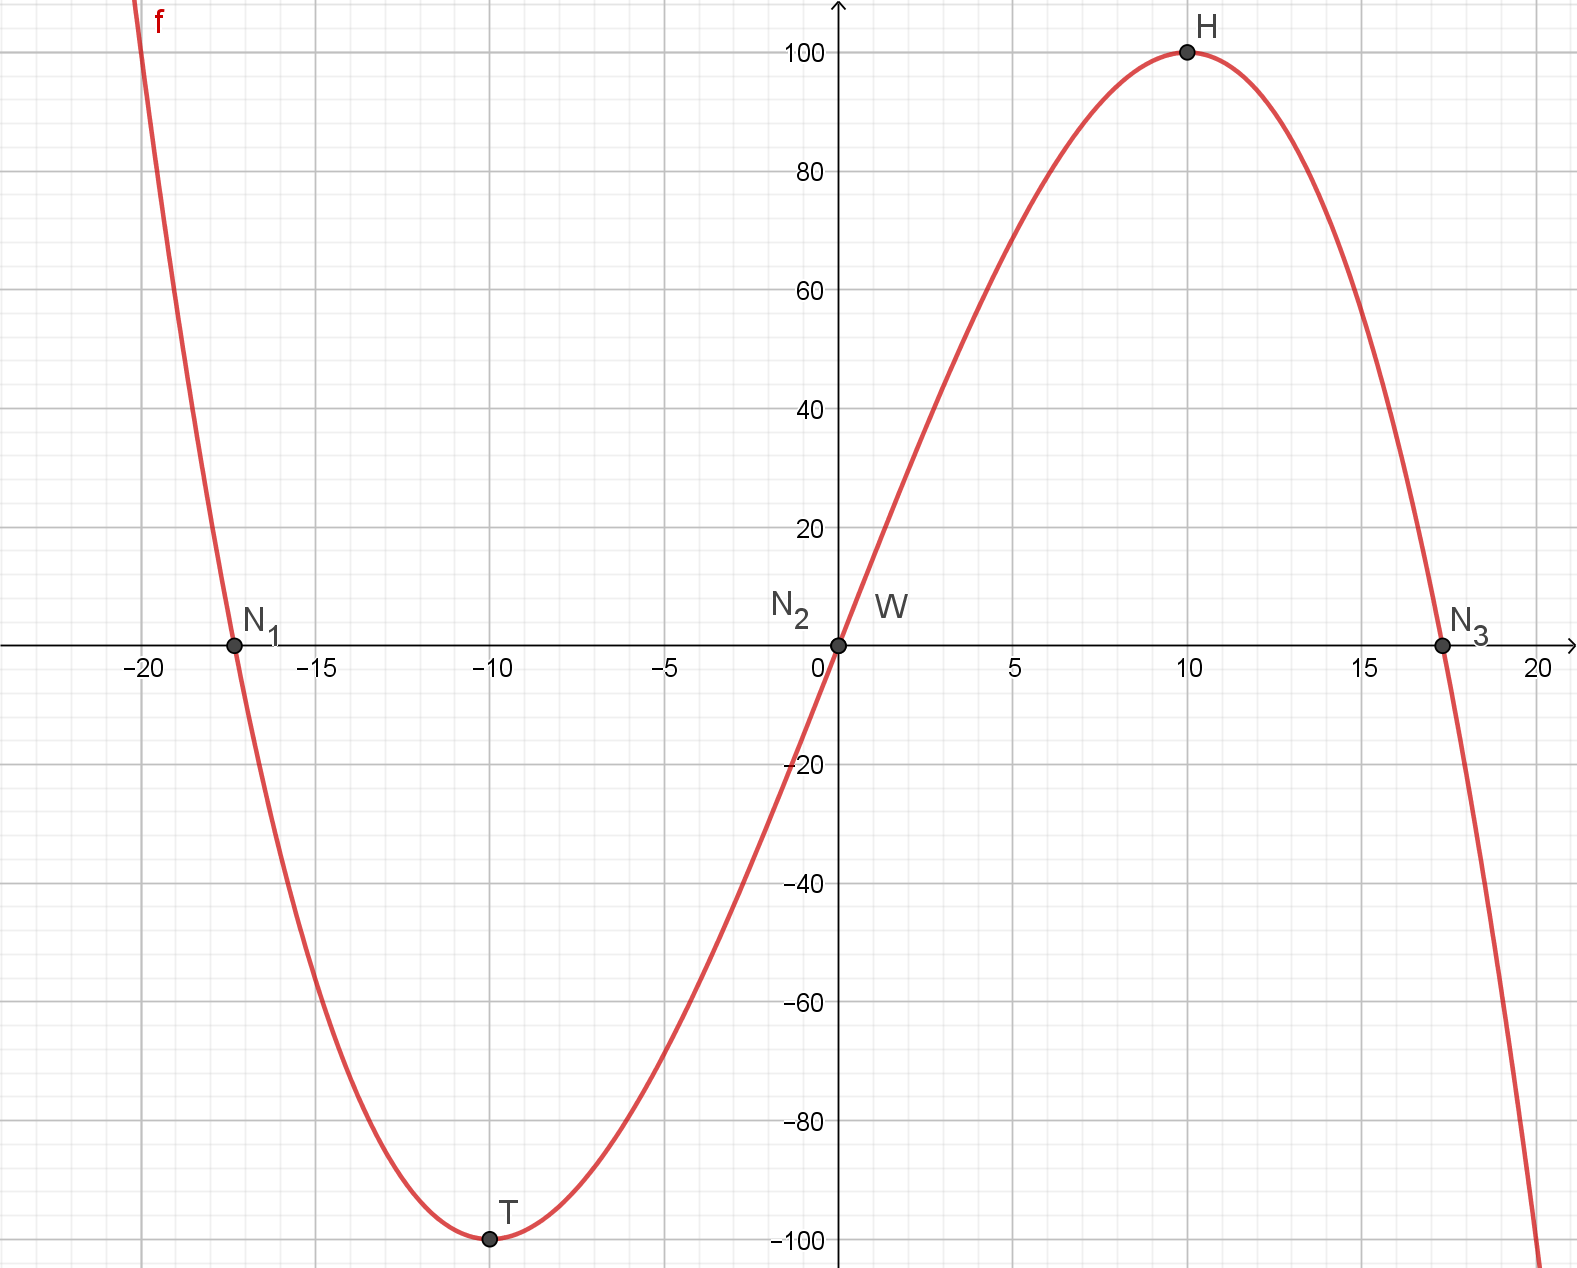
\includegraphics[scale=0.5]{Bilder/HAa.png}
		\end{framed}
		\newpage
		\begin{framed}
			\noindent
			\textbf{(b)} \(\mathbf{f(x) = \frac{1}{9}x^3 -\frac{1}{6}x^2 -2x}\)\\
			\(\Rightarrow f'(x) = \frac{3}{9}x^2 -\frac{2}{6}x -2\)\\
			\(\Rightarrow f''(x) = \frac{6}{9}x - \frac{2}{6}\)\\
			\par\noindent
			\begin{tabularx}{\textwidth}{lXXl}
				(1) & Nullstellen & \(\Rightarrow f(x) = 0\)\\
				\hline\\
				& \(\frac{1}{9}x^3 -\frac{1}{6}x^2 -2x = 0\) & \(\Rightarrow x\) ausklammern\\
				& \( x(\frac{1}{9}x^2 -\frac{1}{6}x -2) = 0\) & \(\Leftrightarrow\) \colorbox{green!10}{\(x_1 = 0\)} oder \(\frac{1}{9}x^2 -\frac{1}{6}x -2 = 0\)\\
				& & \(\frac{1}{9}x^2 -\frac{1}{6}x -2 = 0\) & |\(\cdot9\)\\
				& & \(x^2 \underbrace{-\frac{9}{6}}_{p}x \underbrace{-18}_{q} = 0\) & |pq-Formel\\
				& & \(x_{2,3} = -\frac{-\frac{9}{6}}{2} \pm \sqrt{\left(\frac{-\frac{9}{6}}{2}\right)^2 +18}\) & |\(x_2,x_3\) bestimmen\\
				& & \multicolumn{2}{l}{\colorbox{green!10}{\(x_2\)} \(= -\frac{-\frac{9}{6}}{2} + \sqrt{\left(\frac{-\frac{9}{6}}{2}\right)^2 +18}\) \colorbox{green!10}{\(= 5,06\)}}\\
				& & \multicolumn{2}{l}{und \colorbox{green!10}{\(x_3\)} \(= -\frac{-\frac{9}{6}}{2} - \sqrt{\left(\frac{-\frac{9}{6}}{2}\right)^2 +18}\) \colorbox{green!10}{\(=-3,56\)}}\\
				\multicolumn{4}{l}{Nullstellen: \colorbox{blue!5}{\(N_1(-3,56|0), N_2(0|0)\)} und \colorbox{blue!5}{\(N_3(5,06|0)\)}}\\
				\hline\hline\\
			\end{tabularx}
			\begin{tabularx}{\textwidth}{lXXl}
				(2) & Extremstellen & \(\Rightarrow f'(x) = 0\)\\
				\hline\\
				& \(\frac{3}{9}x^2 -\frac{2}{6}x -2 = 0\) & |\(\cdot 9\)\\
				& \(3x^2 -\frac{18}{6}x -18 = 0\) & |\(:3\)\\
			\end{tabularx}
			\begin{tabularx}{\textwidth}{lXXl}
				& \(x^2 \underbrace{-1}_{p}x \underbrace{-6}_{q} = 0\) & |pq-Formel\\
				& \(x_{4,5} = -\frac{-1}{2} \pm \sqrt{\left(\frac{-1}{2}\right)^2 + 6}\)\\
				& \multicolumn{2}{l}{\colorbox{green!10}{\(x_4\)} \(= -\frac{-1}{2} + \sqrt{\left(\frac{-1}{2}\right)^2 + 6}\) \colorbox{green!10}{\(= -2\)}}\\
				& \multicolumn{2}{l}{und \colorbox{green!10}{\(x_5\)} \(= -\frac{-1}{2} - \sqrt{\left(\frac{-1}{2}\right)^2 + 6}\) \colorbox{green!10}{\(= 3\)}}\\
				\\
				(3) & Art der Extremstelle bestimmen & \(\Rightarrow f''(x_4)\) und \(f''(x_5)\)\\
				\hline\\				 
				& \(f''(-2) = \frac{6}{9}*(-2) - \frac{2}{6} = -\frac{5}{3}< 0\) & \(\Rightarrow\) \colorbox{green!10}{\(x_4\) ist HOP}\\
				& \(f''(3) = \frac{6}{9}*3 - \frac{2}{6} = \frac{5}{3} > 0\) & \(\Rightarrow\) \colorbox{green!10}{\(x_5\) ist TIP}\\
			\end{tabularx}
			\begin{tabularx}{\textwidth}{ll}
				& Die dazugehörigen Punkte bestimmt man mit \(f(x_4)\) bzw. \(f(x_5)\).\\
				& \(f(x_4) = \frac{1}{9}*(-2)^3 -\frac{1}{6}*(-2)^2 -2*(-2) = \frac{22}{9}\)\\
				& \(f(x_5) = \frac{1}{9}*3^3 -\frac{1}{6}*3^2 -2*3 = -4,5\)\\
			\end{tabularx}
			\begin{tabularx}{\textwidth}{ll}
				\multicolumn{2}{l}{So ergeben sich \colorbox{blue!5}{\(T(3|-4,5)\)} und \colorbox{blue!5}{\(H(-2|\frac{22}{9})\)}}\\
			\end{tabularx}
			\begin{tabularx}{\textwidth}{lXXl}
				\hline\hline\\
				(4) & Wendestellen & \(\Rightarrow f''(x) = 0\)\\
				\hline\\
				& \(\frac{6}{9}x - \frac{2}{6} = 0\) & |\(+\frac{2}{6}\)\\
				& \(\frac{6}{9}x = \frac{2}{6}\) & |\(\cdot9\)\\
				& \(6x = \frac{18}{6}\) & |\(:6\)\\
				& \(x = \frac{18}{36} = \frac{1}{2}\) & \(\Rightarrow\) \colorbox{green!10}{\(x_6 = \frac{1}{2}\)}\\
				& Den dazugehörigen Punkt bestimmt man mit \(f(x_6)\).\\
				& \(f(x_6) = \frac{1}{9}*\frac{1}{2}^3 -\frac{1}{6}*\frac{1}{2}^2 -2*\frac{1}{2} = 1\)\\
				\multicolumn{2}{l}{So ergibt sich \colorbox{blue!5}{\(W(\frac{1}{2}|-1)\)}.}\\
				\hline\hline\\
				(5) & Verhalten für große x-Werte\\
				\hline\\
				& Betrachte dafür: \(\frac{1}{9}x^3\)\\
				& \colorbox{green!10}{\(\frac{1}{9}x^3\xrightarrow{x\rightarrow-\infty}-\infty\)} & \colorbox{green!10}{\(\frac{1}{9}x^3\xrightarrow{x\rightarrow\infty}\infty\)}\\
				\hline\hline\\
			\end{tabularx}\\
			\par\noindent
			Der Funktionsgraph sieht wie folgt aus:\\
			\par
			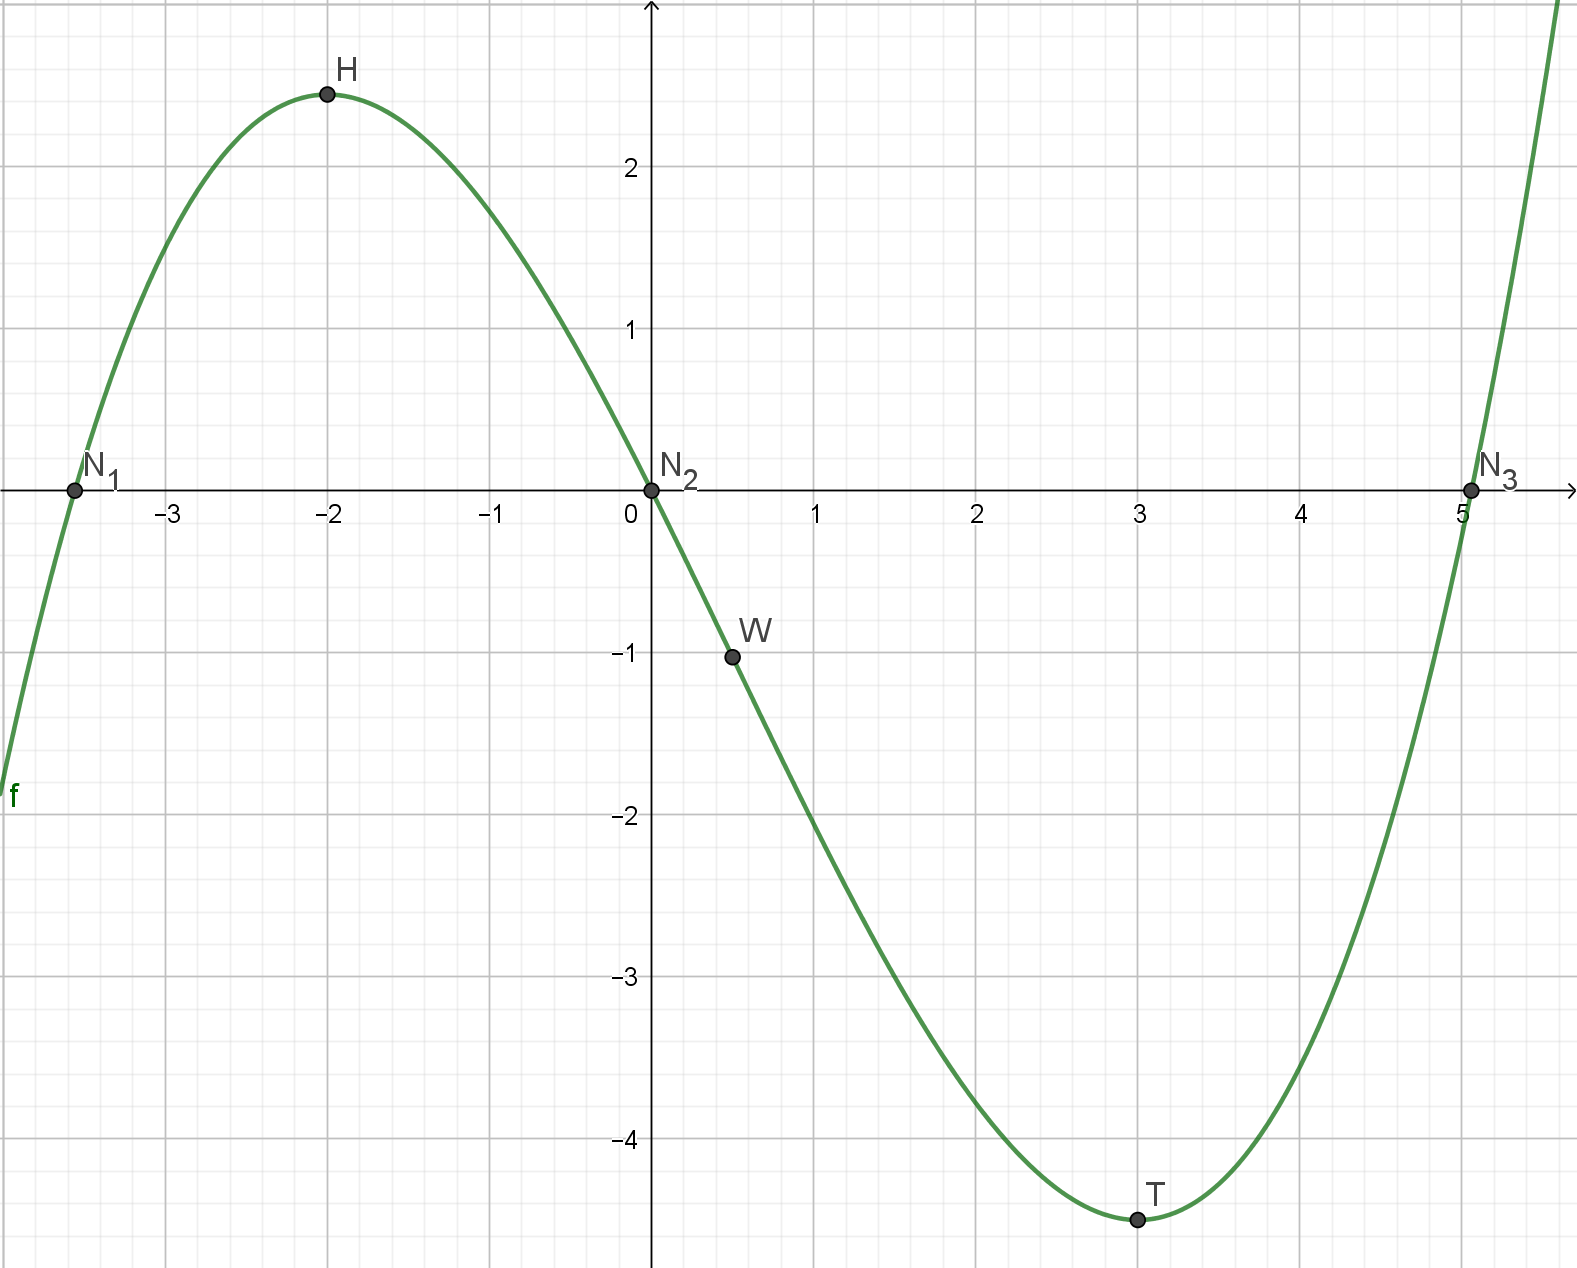
\includegraphics[scale=0.4]{Bilder/HAb.png}
		\end{framed}
		\newpage
		\begin{framed}
			\noindent
			\textbf{(c)} \(\mathbf{f(x) = x^3 -6x^2 +9x}\)\\
			\(\Rightarrow f'(x) = 3x^2 -12x+9\)\\
			\(\Rightarrow f''(x) = 6x -12\)\\
			\par\noindent
			\begin{tabularx}{\textwidth}{lXXl}
				(1) & Nullstellen & \(\Rightarrow f(x) = 0\)\\
				\hline\\
				& \(x^3 -6x^2 + 9x = 0\) & \(\Rightarrow x\) ausklammern\\
				& \(x(x^2 -6x +9) = 0\) & \(\Leftrightarrow\) \colorbox{green!10}{\(x_1 = 0\)} oder \(x^2 -6x+9 = 0\)\\
				\cline{1-2}\\
				& \(x^2 \underbrace{-6}_{p}x +\underbrace{9}_{q} = 0\) & |pq-Formel\\
				& & \(x_{2,3} = -\frac{-6}{2} \pm \sqrt{\left(\frac{-6}{2}\right)^2 -9}\) & |\(x_2,x_3\) bestimmen\\
				& & \multicolumn{2}{l}{\colorbox{green!10}{\(x_2\)} \(= -\frac{-6}{2} + \sqrt{\left(\frac{-6}{2}\right)^2 -9}\) \colorbox{green!10}{\(= 3\)}}\\
				& & \multicolumn{2}{l}{und \colorbox{green!10}{\(x_3\)} \(= -\frac{-6}{2} - \sqrt{\left(\frac{-6}{2}\right)^2 -9}\) \colorbox{green!10}{\(=3\)}}\\
				\multicolumn{4}{l}{Nullstellen: \colorbox{blue!5}{\(N_1(0|0)\)} und \colorbox{blue!5}{\(N_2(3|0)\)}}\\
				\hline\hline\\
			\end{tabularx}
			\begin{tabularx}{\textwidth}{lXXl}
				(2) & Extremstellen & \(\Rightarrow f'(x) = 0\)\\
				\hline\\
				& \(3x^2 -12x+9 = 0\) & |\(:3\)\\
				& \(x^2 \underbrace{-4}_{p}x +\underbrace{3}_{q} = 0\) & |pq-Formel\\
				& & \(x_{3,4} = -\frac{-4}{2} \pm \sqrt{\left(\frac{-4}{2}\right)^2 -3}\) & |\(x_3,x_4\) bestimmen\\
				& & \multicolumn{2}{l}{\colorbox{green!10}{\(x_3\)} \(= -\frac{-4}{2} + \sqrt{\left(\frac{-4}{2}\right)^2 -3}\) \colorbox{green!10}{\(= 3\)}}\\
				& & \multicolumn{2}{l}{und \colorbox{green!10}{\(x_4\)} \(= -\frac{-4}{2} \pm \sqrt{\left(\frac{-4}{2}\right)^2 -3}\) \colorbox{green!10}{\(= 1\)}}\\
				\\
				(3) & Art der Extremstelle bestimmen & \(\Rightarrow f''(x_3)\) und \(f''(x_4)\)\\
				\hline\\				 
				& \(f''(3) =  6*3 -12 = 6 > 0\) & \(\Rightarrow\) \colorbox{green!10}{\(x_3\) ist TIP}\\
				& \(f''(1) = 6*1 -12 = -6 < 0\) & \(\Rightarrow\) \colorbox{green!10}{\(x_5\) ist HOP}\\
				& \multicolumn{3}{l}{Die dazugehörigen Punkte bestimmt man mit \(f(x_3)\) bzw. \(f(x_4)\).}\\
				& \multicolumn{2}{l}{\(f(x_3) = 3^3 -6*3^2 +9*3 = 0\)}\\
				& \multicolumn{2}{l}{\(f(x_4) = 1^3 -6*1^2 +9*1 = 4\)}\\
				
			\end{tabularx}
			\begin{tabularx}{\textwidth}{lXXl}
				\multicolumn{2}{l}{So ergeben sich \colorbox{blue!5}{\(T(3|0) = N_2(3|0)\)} und \colorbox{blue!5}{\(H(1|4)\)}}\\
				\hline\hline\\
				(4) & Wendestellen & \(\Rightarrow f''(x) = 0\)\\
				\hline\\
				& \(6x -12 = 0\) & |\(+12\)\\
				& \(6x = 12\) & |\(:2\)\\
				& \(x = 2\) & \(\Rightarrow\) \colorbox{green!10}{\(x_5 = 2\)}\\
				& Den dazugehörigen Punkt bestimmt man mit \(f(x_5)\).\\
				& \(f(x_5) = 2^3 -6*2^2 +9*2 = 2\)\\
				\multicolumn{2}{l}{So ergibt sich \colorbox{blue!5}{\(W(2|2)\)}.}\\
				\hline\hline\\
				(5) & Verhalten für große x-Werte\\
				\hline\\
				& Betrachte dafür: \(x^3\)\\
				& \colorbox{green!10}{\(x^3\xrightarrow{x\rightarrow-\infty}-\infty\)} & \colorbox{green!10}{\(x^3\xrightarrow{x\rightarrow\infty}\infty\)}\\
				\hline\hline\\
			\end{tabularx}\\
			\par\noindent
			Der Funktionsgraph sieht wie folgt aus:\\
			\par
			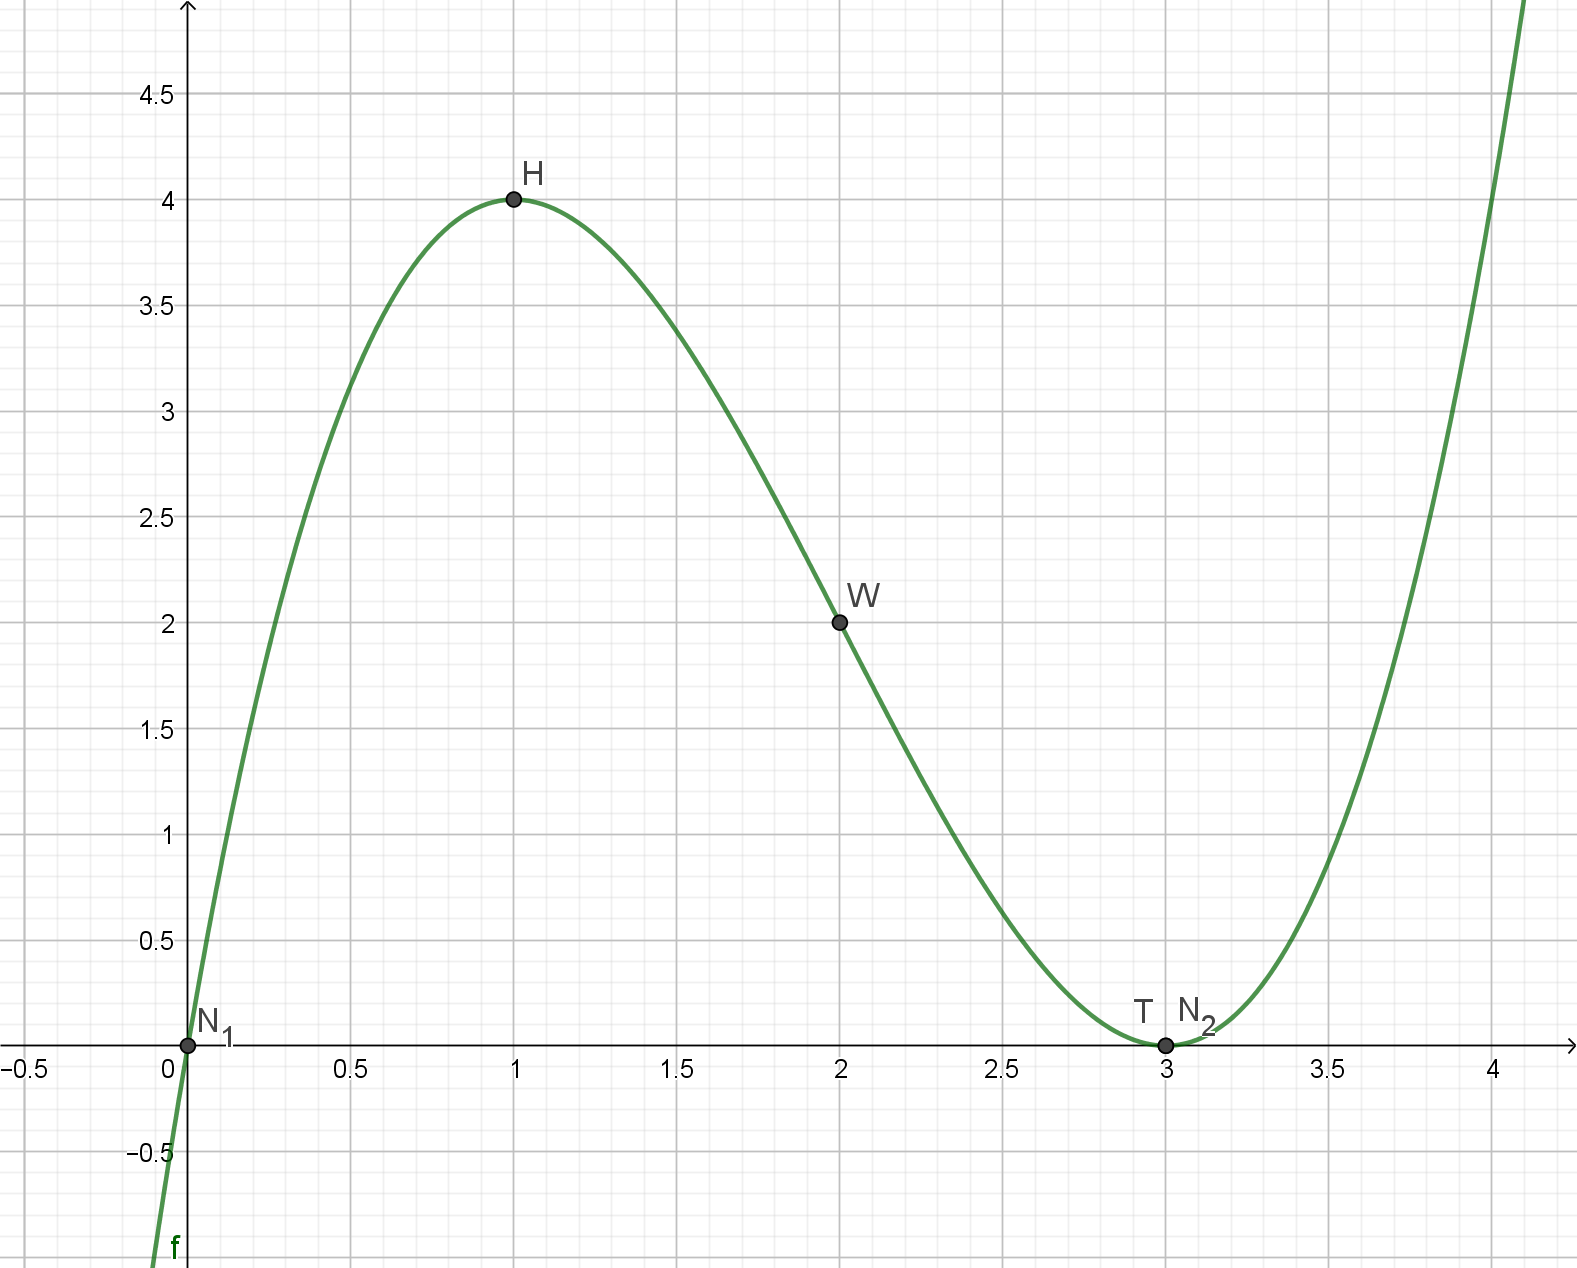
\includegraphics[scale=0.4]{Bilder/HAc.png}
		\end{framed}
		\newpage
		\begin{framed}
			\noindent
			\textbf{(d)} \(\mathbf{f(x) = x^3 +4x^2-11x-30}\)\\
			\(\Rightarrow f'(x) = 3x^2 +8x-11\)\\
			\(\Rightarrow f''(x) = 6x +8\)\\
			\par\noindent
			\begin{tabularx}{\textwidth}{lXXl}
				(1) & Nullstellen & \(\Rightarrow f(x) = 0\)\\
				\hline\\
				& \(x^3 +4x^2-11x-30 = 0\) & Nullstelle raten \colorbox{green!10}{\(x_1 = -2\)}\\
				& \(f(-2) = (-2)^3 +4*(-2)^2-11*(-2)-30 = 0\)\\
				& Polynomdivision \(f(x):\underbrace{(x+2)}_{(x-NST)}\)\\
			\end{tabularx}
			\polyset{style=C, div=:,vars=x}
			\polylongdiv{x^3+4x^2-11x-30}{x+2}\\
			\begin{tabularx}{\textwidth}{lXXl}
				& \multicolumn{3}{l}{\(f(x) = x^3 +4x^2-11x-30 = (x+2)*(x^2+2x-15) = 0\)}\\
				& & \multicolumn{2}{l}{\(\Leftrightarrow\) \colorbox{green!10}{\(\underbrace{x+2=0}_{x_1=-2}\)} oder \(x^2 +2x-15 = 0\)}\\
				\cline{1-2}\\
				& \(x^2 +\underbrace{2}_{p}x \underbrace{-15}_{q} = 0\) & |pq-Formel\\
				& & \(x_{2,3} = -\frac{2}{2} \pm \sqrt{\left(\frac{2}{2}\right)^2 +15}\) & |\(x_2,x_3\) bestimmen\\
				& & \multicolumn{2}{l}{\colorbox{green!10}{\(x_2\)} \(= -\frac{2}{2} + \sqrt{\left(\frac{2}{2}\right)^2 +15}\) \colorbox{green!10}{\(= 3\)}}\\
				& & \multicolumn{2}{l}{und \colorbox{green!10}{\(x_3\)} \(= -\frac{2}{2} - \sqrt{\left(\frac{2}{2}\right)^2 +15}\) \colorbox{green!10}{\(=-5\)}}\\
				\multicolumn{4}{l}{Nullstellen: \colorbox{blue!5}{\(N_1(-5|0), N_2(-2|0)\)} und \colorbox{blue!5}{\(N_3(3|0)\)}}\\
				\hline\hline\\
				(2) & Extremstellen & \(\Rightarrow f'(x) = 0\)\\
				\hline\\
				& \(3x^2 +8x-11 = 0\) & |\(:3\)\\
				& \(x^2 +\underbrace{\frac{8}{3}}_{p}x \underbrace{-\frac{11}{3}}_{q} = 0\) & |pq-Formel\\
				& & \(x_{3,4} = -\frac{\frac{8}{3}}{2} \pm \sqrt{\left(\frac{\frac{8}{3}}{2}\right)^2 +\frac{11}{3}}\) & |\(x_4,x_5\) bestimmen\\
			\end{tabularx}
			\begin{tabularx}{\textwidth}{lXXl}
				& & \multicolumn{2}{l}{\colorbox{green!10}{\(x_5\)} \(= -\frac{\frac{8}{3}}{2} + \sqrt{\left(\frac{\frac{8}{3}}{2}\right)^2 +\frac{11}{3}}\) \colorbox{green!10}{\(= 1\)}}\\
				& & \multicolumn{2}{l}{und \colorbox{green!10}{\(x_5\)} \(= -\frac{\frac{8}{3}}{2} - \sqrt{\left(\frac{\frac{8}{3}}{2}\right)^2 +\frac{11}{3}}\) \colorbox{green!10}{\(= -\frac{11}{3}\)}}\\
				\\
				(3) & Art der Extremstelle bestimmen & \(\Rightarrow f''(x_4)\) und \(f''(x_5)\)\\
				\hline\\				 
				& \multicolumn{2}{l}{\(f''(1) =  6*1 +8 = 14 > 0\)} & \(\Rightarrow\) \colorbox{green!10}{\(x_3\) ist TIP}\\
				& \multicolumn{2}{l}{\(f''(-\frac{11}{3}) = 6*(-\frac{11}{3}) + 8 = -14 < 0\)} & \(\Rightarrow\) \colorbox{green!10}{\(x_5\) ist HOP}\\
				& \multicolumn{3}{l}{Die dazugehörigen Punkte bestimmt man mit \(f(x_3)\) bzw. \(f(x_4)\).}\\
			\end{tabularx}
			\begin{tabularx}{\textwidth}{ll}
				& \(f(x_4) = 1^3 +4*1^2-11*1-30 = -36\)\\
				& \(f(x_5) = (-\frac{11}{3})^3 +4*(-\frac{11}{3})^2-11*(-\frac{11}{3})-30 = 14,81\)\\
				\multicolumn{2}{l}{So ergeben sich \colorbox{blue!5}{\(T(1|-36)\)} und \colorbox{blue!5}{\(H(-\frac{11}{3}|14,81)\)}}\\
				\hline\hline\\
			\end{tabularx}
			\begin{tabularx}{\textwidth}{lXXl}
				(4) & Wendestellen & \(\Rightarrow f''(x) = 0\)\\
				\hline\\
				& \(6x +8 = 0\) & |\(-8\)\\
				& \(6x = -8\) & |\(:6\)\\
				& \(x = -\frac{8}{6} = -\frac{4}{3}\) & \(\Rightarrow\) \colorbox{green!10}{\(x_6 = -\frac{4}{3}\)}\\
				& Den dazugehörigen Punkt bestimmt man mit \(f(x_6)\).\\
				& \(f(x_5) = (-\frac{4}{3})^3 +4*(-\frac{4}{3})^2-11*(-\frac{4}{3})-30 = -10,59\)\\
				\multicolumn{2}{l}{So ergibt sich \colorbox{blue!5}{\(W(-\frac{4}{3}|-10,59)\)}.}\\
				\hline\hline\\
				(5) & Verhalten für große x-Werte\\
				\hline\\
				& Betrachte dafür: \(x^3\)\\
				& \colorbox{green!10}{\(x^3\xrightarrow{x\rightarrow-\infty}-\infty\)} & \colorbox{green!10}{\(x^3\xrightarrow{x\rightarrow\infty}\infty\)}\\
				\hline\hline\\
			\end{tabularx}\\
			\newpage
			Der Funktionsgraph sieht wie folgt aus:\\
			\par
			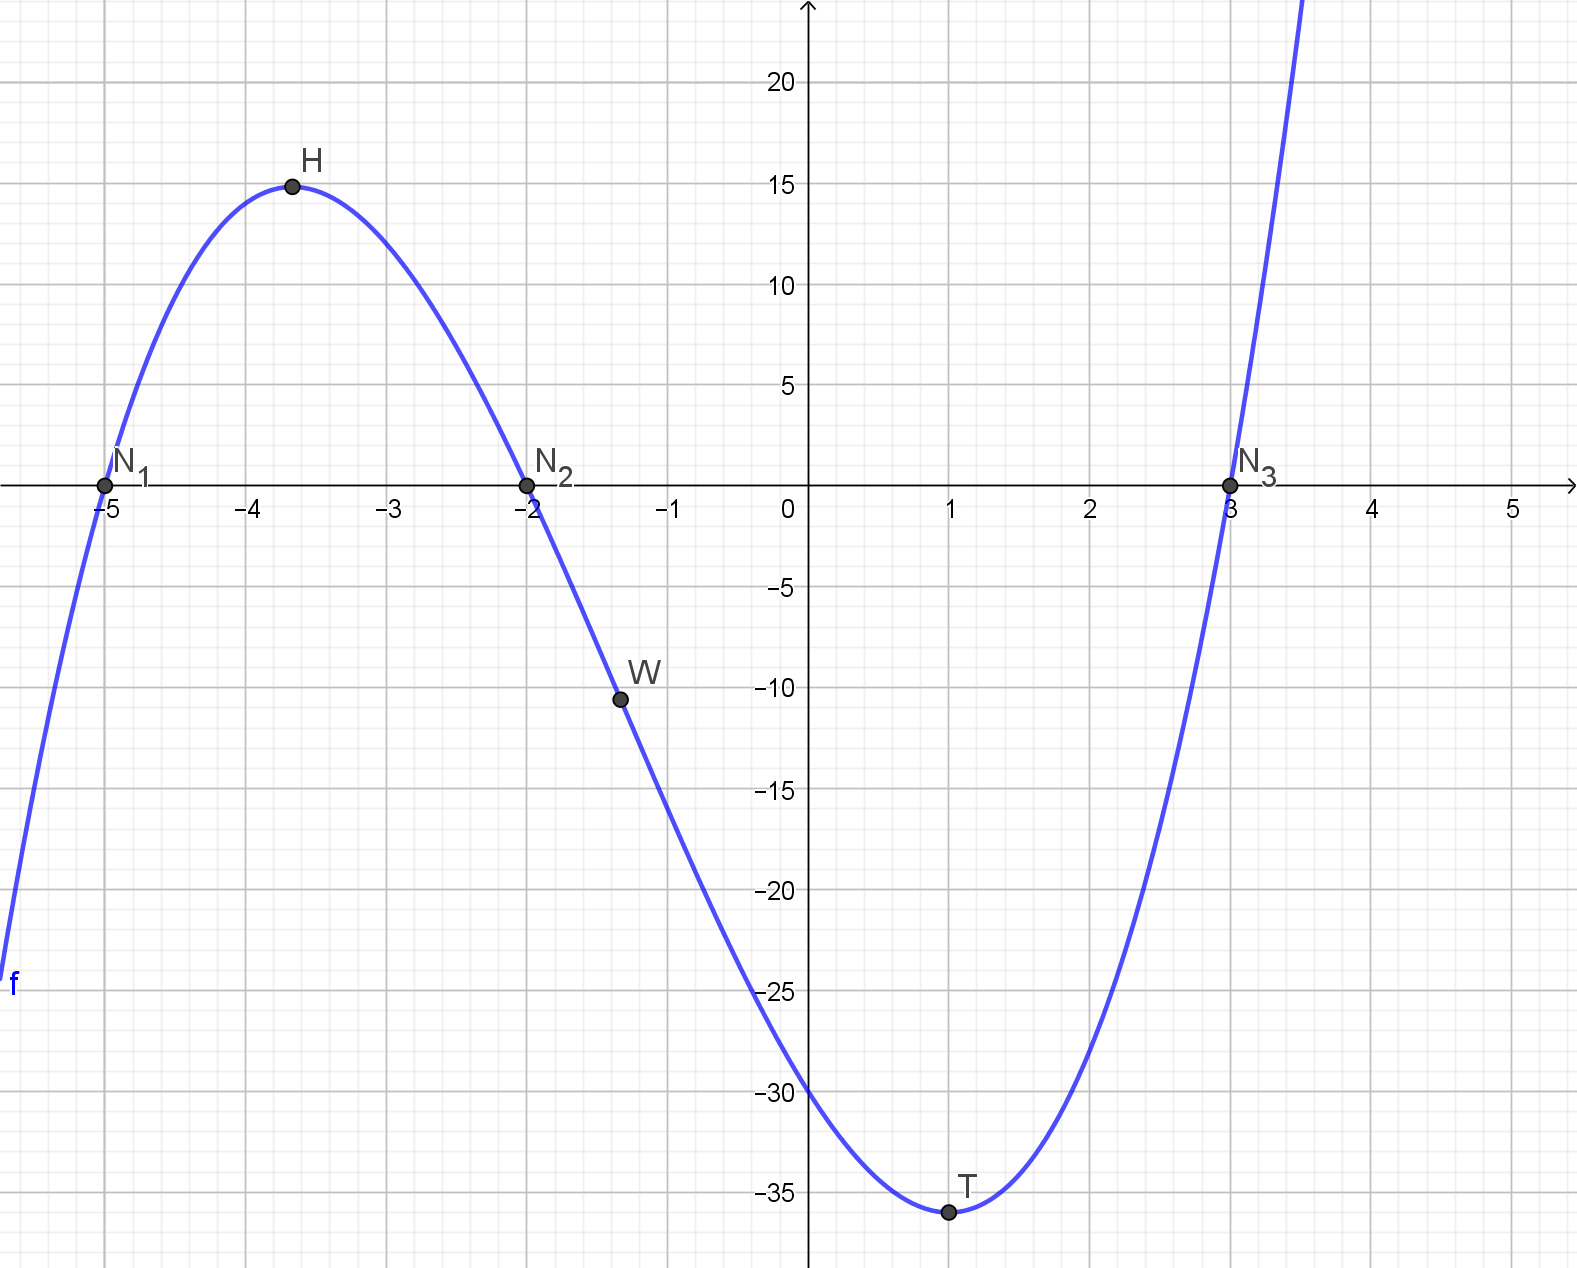
\includegraphics[scale=0.4]{Bilder/HAd.png}\\
		\end{framed}
		\newpage
		\begin{framed}
			\noindent
			\textbf{(e)} \(\mathbf{f(x) = -x^4 +24x^2-80}\)\\
			\(\Rightarrow f'(x) = -4x^3+48x\)\\
			\(\Rightarrow f''(x) = -12x^2+48\)\\
			\par\noindent
			\begin{tabularx}{\textwidth}{lXXl}
				(1) & Nullstellen & \(\Rightarrow f(x) = 0\)\\
				\hline\\
				& \(-x^4 +24x^2-80 = 0\) & Substitution \(\Rightarrow z = x^2\)\\
				& \(-\underbrace{z^2}_{x^2\cdot x^2} + 24\underbrace{z}_{x^2} -80 = 0\)\\
				& \(-z^2  +24z -80 = 0\) & |\(\cdot(-1)\)\\
				& \(z^2  \underbrace{-24}_{p}z +\underbrace{80}_{q} = 0\) & |pq-Formel\\
				& & \(z_{1,2} = -\frac{-24}{2} \pm \sqrt{\left(\frac{-24}{2}\right)^2 -80}\) & |\(z_1,z_2\) bestimmen\\
				& & \multicolumn{2}{l}{\colorbox{green!10}{\(z_1\)} \(= \frac{24}{2} + \sqrt{\left(\frac{-24}{2}\right)^2 +80}\) \colorbox{green!10}{\(= 20\)}}\\
				& & \multicolumn{2}{l}{und \colorbox{green!10}{\(z_2\)} \(= \frac{24}{2} - \sqrt{\left(\frac{-24}{2}\right)^2 +80}\) \colorbox{green!10}{\(=4\)}}\\
				\multicolumn{4}{l}{\textit{Rücksubstitution} \(\Rightarrow z = x^2\)}\\
			\end{tabularx}
			\begin{tabularx}{\textwidth}{lXlXl}
				& \(x^2_1 = z_1 = 20\) & | \(\sqrt{}\) & \(x^2_2 = z_2 = 4\) &| \(\sqrt{}\)\\
				& \colorbox{blue!5}{\(x_{1_{1}} = \sqrt{20} = 4,47\)} & & \colorbox{blue!5}{\(x_{2_{1}} = \sqrt{4} = 2\)}\\
				& \colorbox{blue!5}{\(x_{1_{2}} = \sqrt{20} = -4,47\)} & & \colorbox{blue!5}{\(x_{2_{2}} = \sqrt{4} = -2\)}\\
			\end{tabularx}
			\begin{tabularx}{\textwidth}{lXXl}
				\multicolumn{4}{l}{Nullstellen: \colorbox{blue!5}{\(N_1(-4,47|0), N_2(-2|0), N_3(2|0)\)} und \colorbox{blue!5}{\(N_4(4,47|0)\)}}\\
				\hline\hline\\
				(2) & Extremstellen & \(\Rightarrow f'(x) = 0\)\\
				\hline\\
				& \(-4x^3+48x = 0\) & \(\Rightarrow x\) ausklammern\\
				& \(x(-4x^2+48) = 0\) & \(\Leftrightarrow \) \colorbox{blue!5}{\(x_5 = 0\)} oder \(-4x^2+48 = 0\)\\
				& & \(-4x^2+48 = 0\) & | \(+4x^2\)\\
				& & \(48 = 4x^2\) & |\(:4\)\\
				& & \(12 = x^2\) & |\(\sqrt{}\)\\
				& & \colorbox{blue!5}{\(x_6 = 3,46\)} und \colorbox{blue!5}{\(x_7 = -3,46\)}\\
				\\
				(3) & Art der Extremstelle bestimmen & \(\Rightarrow f''(x_5), f(x_6)\) und \(f''(x_7)\)\\
				\hline\\				 
				& \multicolumn{2}{l}{\(f''(0) =  -12*0^2+48 = 48> 0\)} & \(\Rightarrow\) \colorbox{green!10}{\(x_5\) ist TIP}\\
				& \multicolumn{2}{l}{\(f''(3,46) =  -12*(3,46)^2 +48 = -95,66< 0\)} & \(\Rightarrow\) \colorbox{green!10}{\(x_6\) ist HOP}\\
				& \multicolumn{2}{l}{\(f''(-3,46) = -12*(-3,46)^2 +48 = -95,66 < 0\)} & \(\Rightarrow\) \colorbox{green!10}{\(x_7\) ist HOP}\\
				& \multicolumn{3}{l}{Die dazugehörigen Punkte bestimmt man mit \(f(x_5), f(x_6)\) bzw. \(f(x_7)\).}\\
			\end{tabularx}
			\begin{tabularx}{\textwidth}{ll}
				& \(f(x_5) = -0^4 +24*0^2-80 = -80\)\\
				& \(f(x_6) = -3,46^4 +24*(3,46)^2-80 = 64\)\\
				& \(f(x_7) = -(-3,46)^4 +24*(-3,46)^2-80 = 64\)\\
				\multicolumn{2}{l}{So ergeben sich \colorbox{blue!5}{\(T(0|-80)\)} und \colorbox{blue!5}{\(H_1(-3,46|64)\)} und \colorbox{blue!5}{\(H_2(3,46|64)\)}}\\
				\hline\hline\\
			\end{tabularx}
			\begin{tabularx}{\textwidth}{lXXl}
				(4) & Wendestellen & \(\Rightarrow f''(x) = 0\)\\
				\hline\\
				& \(-12*x^2+48 = 0\) & |\(+12x^2\)\\
				& \(48 = 12x^2\) & |\(:12\)\\
				& \(4 = x^2\) & |\(\sqrt{}\)\\
				& \colorbox{green!10}{\(x_8 = 3,46 = N_3\)} und \colorbox{blue!5}{\(x_9 = -3,46 = N_2\)}\\
				& Die dazugehörigen Punkte haben wir in (1) bereits bestimmt.\\
				\multicolumn{2}{l}{So ergibt sich \colorbox{blue!5}{\(W_1(-3,46|0)\)} und \colorbox{blue!5}{\(W_2(3,46|0)\)}}\\
				\hline\hline\\
				(5) & Verhalten für große x-Werte\\
				\hline\\
				& Betrachte dafür: \(-x^4\)\\
				& \colorbox{green!10}{\(-x^4\xrightarrow{x\rightarrow-\infty}-\infty\)} & \colorbox{green!10}{\(-x^4\xrightarrow{x\rightarrow\infty}-\infty\)}\\
				\hline\hline\\
			\end{tabularx}\\
			Der Funktionsgraph sieht wie folgt aus:\\
			\par
			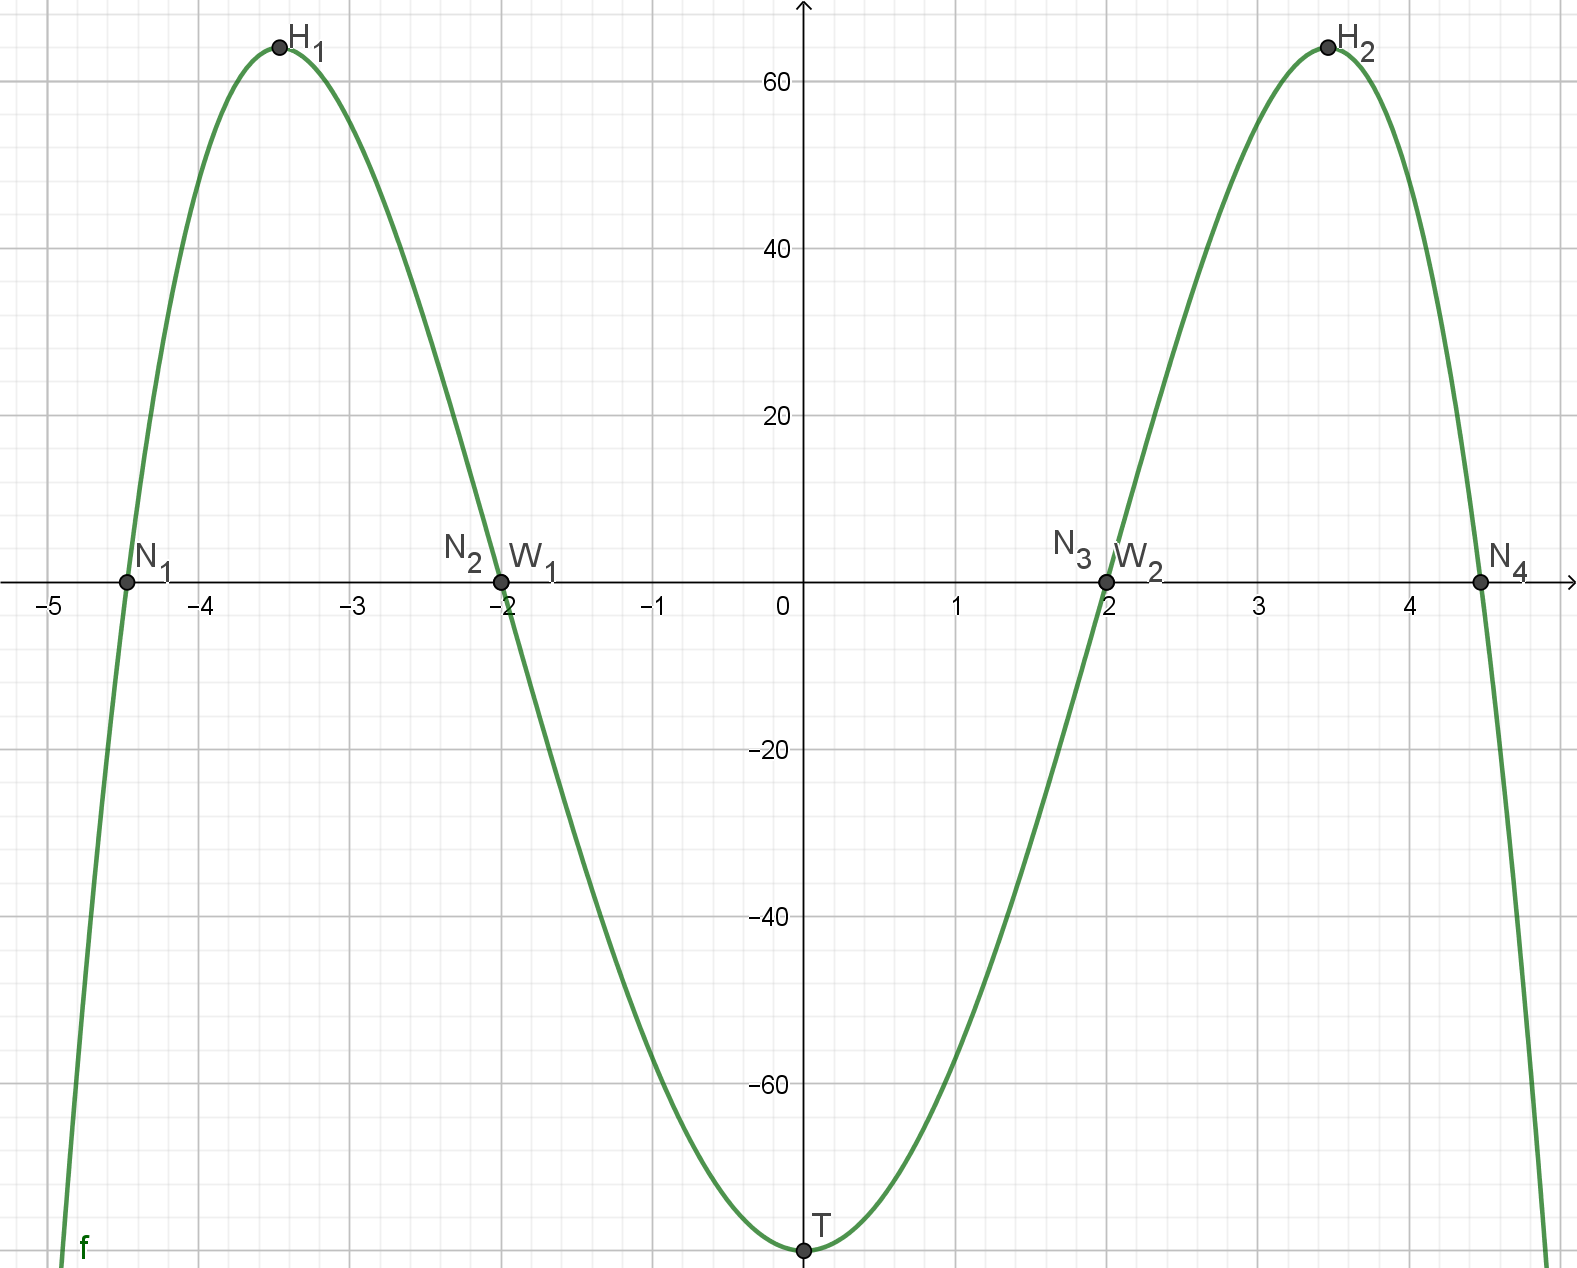
\includegraphics[scale=0.35]{Bilder/HAe.png}\\
		\end{framed}
		\newpage
		\begin{framed}
			\noindent
			\textbf{(f)} \(\mathbf{f(x) = \frac{1}{8}x^4 -x^2+2}\)\\
			\(\Rightarrow f'(x) = \frac{1}{2}x^3-2x\)\\
			\(\Rightarrow f''(x) = \frac{3}{4}x^2 -2\)\\
			\par\noindent
			\begin{tabularx}{\textwidth}{lXXl}
				(1) & Nullstellen & \(\Rightarrow f(x) = 0\)\\
				\hline\\
				& \(\frac{1}{8}x^4 -x^2+2 = 0\) & Substitution \(\Rightarrow z = x^2\)\\
				& \(\frac{1}{8}\underbrace{z^2}_{x^2\cdot x^2} \underbrace{z}_{x^2} +2 = 0\)\\
				& \(\frac{1}{8}z^2  -z +2 = 0\) & |\(\cdot 8\)\\
				& \(z^2  \underbrace{-8}_{p}z +\underbrace{16}_{q} = 0\) & |pq-Formel\\
				& & \(z_{1,2} = -\frac{-8}{2} \pm \sqrt{\left(\frac{-8}{2}\right)^2 -16}\) & |\(z_1,z_2\) bestimmen\\
				& & \multicolumn{2}{l}{\colorbox{green!10}{\(z_1\)} \(= \frac{8}{2} + \sqrt{\left(\frac{-8}{2}\right)^2 -16}\) \colorbox{green!10}{\(= 4\)}}\\
				& & \multicolumn{2}{l}{und \colorbox{green!10}{\(z_2\)} \(= \frac{8}{2} - \sqrt{\left(\frac{-8}{2}\right)^2 -16}\) \colorbox{green!10}{\(=4 = z_1\)}}\\
				\multicolumn{4}{l}{\textit{Rücksubstitution} \(\Rightarrow z = x^2\)}\\
				& \(x^2_1 = z_1 = 4\) & |\(\sqrt{}\)\\
				& \colorbox{blue!5}{\(x_{1} = \sqrt{4} = 2\)}\\
				& \colorbox{blue!5}{\(x_{2} = \sqrt{4} = -2\)}\\
				\multicolumn{4}{l}{Nullstellen: \colorbox{blue!5}{\(N_1(-2|0)\)} und \colorbox{blue!5}{\(N_2(2|0)\)}}\\
				\hline\hline\\
				(2) & Extremstellen & \(\Rightarrow f'(x) = 0\)\\
				\hline\\
				& \(\frac{1}{2}x^3-2x = 0\) & \(\Rightarrow x\) ausklammern\\
				& \(x(\frac{1}{2}x^2-2) = 0\) & \(\Leftrightarrow \) \colorbox{blue!5}{\(x_3 = 0\)} oder \(\frac{1}{2}x^2-2 = 0\)\\
				& & \(\frac{1}{2}x^2-2 = 0\) & | \(+2\)\\
				& & \(\frac{1}{2}x^2 = 2\) & |\(\cdot 2\)\\
				& & \(x^2 = 4\) & |\(\sqrt{}\)\\
				& & \colorbox{blue!5}{\(x_4 = 2 = N_2\)} und \colorbox{blue!5}{\(x_5 = -2 = N_1\)}\\
				\\
				(3) & Art der Extremstelle bestimmen & \(\Rightarrow f''(x_3), f''(x_4)\) und \(f''(x_5)\)\\
				\hline\\		
				& \multicolumn{2}{l}{\(f''(0) =  \frac{3}{4}0^2 -2 = -2 < 0\)} & \(\Rightarrow\) \colorbox{green!10}{\(x_3\) ist HOP}\\		 
				& \multicolumn{2}{l}{\(f''(2) =  \frac{3}{4}2^2 -2 = 1 > 0\)} & \(\Rightarrow\) \colorbox{green!10}{\(x_4\) ist TIP}\\
				& \multicolumn{2}{l}{\(f''(-2) =  \frac{3}{4}*(-2)^2 -2 = 1 > 0\)} & \(\Rightarrow\) \colorbox{green!10}{\(x_5\) ist TIP}\\
				& \multicolumn{3}{l}{Die dazugehörigen Punkte bestimmt man mit \(f(x_3), f(x_4)\) bzw. \(f(x_5)\).}\\
			\end{tabularx}
			\begin{tabularx}{\textwidth}{ll}
				& \(f(x_3) = \frac{1}{8}0^4 -0^2+2 = 2\)\\
				& \(f(x_4) = \frac{1}{8}\cdot 2^4 -2^2+2 = 0\)\\
				& \(f(x_5) = \frac{1}{8}\cdot (-2)^4 -(-2)^2+2 = 0\)\\
				\multicolumn{2}{l}{So ergeben sich \colorbox{blue!5}{\(H(0|2)\)} und \colorbox{blue!5}{\(T_1(-2|0)\)} und \colorbox{blue!5}{\(T_2(2|0)\)}}\\
				\hline\hline\\
			\end{tabularx}
			\begin{tabularx}{\textwidth}{lXXl}
				(4) & Wendestellen & \(\Rightarrow f''(x) = 0\)\\
				\hline\\
				& \(\frac{3}{4}x^2 -2 = 0\) & |\(+2\)\\
				& \(\frac{3}{4}x^2 = 2\) & |\(\cdot 4\)\\
				& \(3x^2 = 8\) & |\(:3\)\\
				& \(x^2 = \frac{8}{3}\) & | \(\sqrt{}\)\\
				& \colorbox{green!10}{\(x_6 = 1,63\)} und \colorbox{blue!5}{\(x_7 = -1,63\)}\\
				& \multicolumn{2}{l}{Die dazugehörigen Punkte bestimmt man mit \(f(x_6)\) bzw. \(f(x_7)\).}\\
				& \multicolumn{2}{l}{\(f(x_6) = \frac{1}{8}\cdot(1,63)^4 -(1,63)^2+2 = \frac{2}{9} = \frac{1}{8}\cdot(-1,63)^4 -(-1,63)^2+2 = f(x_7)\)}\\
				\multicolumn{2}{l}{So ergibt sich \colorbox{blue!5}{\(W_1(-1,63|\frac{2}{9})\)} und \colorbox{blue!5}{\(W_2(1,63|\frac{2}{9})\)}}\\
				\hline\hline\\
				(5) & Verhalten für große x-Werte\\
				\hline\\
				& Betrachte dafür: \(\frac{1}{8}x^4\)\\
				& \colorbox{green!10}{\(\frac{1}{8}x^4\xrightarrow{x\rightarrow-\infty}\infty\)} & \colorbox{green!10}{\(\frac{1}{8}x^4\xrightarrow{x\rightarrow\infty}\infty\)}\\
				\hline\hline\\
			\end{tabularx}\\
			Der Funktionsgraph sieht wie folgt aus:\\
			\par
			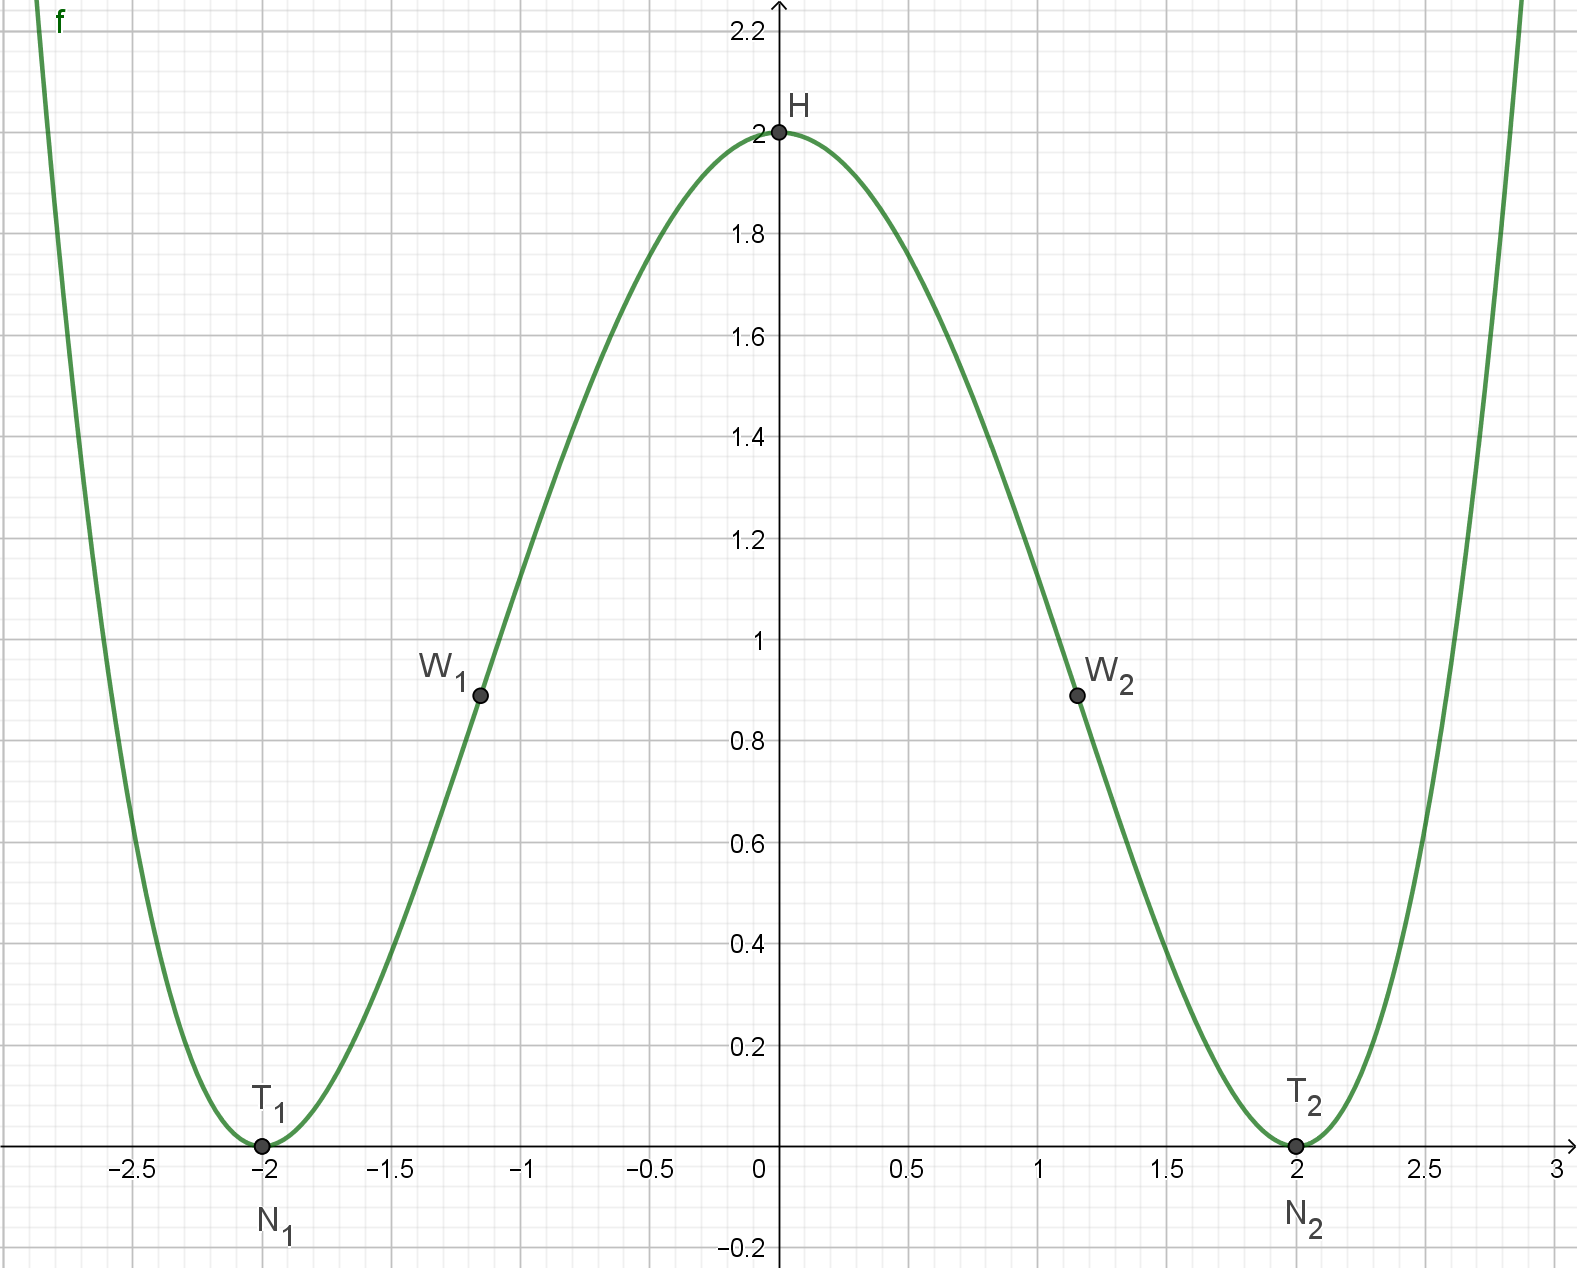
\includegraphics[scale=0.35]{Bilder/HAf.png}\\
		\end{framed}
	\end{worksheet}
\end{document}